\chapter{Проводник в электростатическом поле}

    \begin{definition}
        Проводник -- это твёрдое, жидкое или газообразное тело, у которого есть 
        свободные носители заряда (электроны или ионы), то есть заряды могут 
        свободно перемещаться по всему объёму тела.
    \end{definition}

    К проводникам относят: все металлы (в том числе и ртуть), их сплавы, 
    электролиты и ионизированный газ (плазма).

\section{Поле внутри сплошного проводника}

    \begin{proposition}
        Внутри сплошного проводника поле \( \vec{E} \) в любой точке равно нулю.
    \end{proposition}

    \( \vec{E}_{\textit{индуц}} = -\vec{E}_{\textit{внеш}} \). Если бы
    \( \vec{E}_{\textit{внутр}} \neq 0 \), то в проводнике был бы ток.

    \begin{remark}
        Однако, на создание индуцированных зарядов нужно время, но оно крайне
        мало: \( \tau_{\textit{релакс}} \sim 10^{-15} \text{ с} \).
    \end{remark}

    \begin{figure}[!b]
        \center
        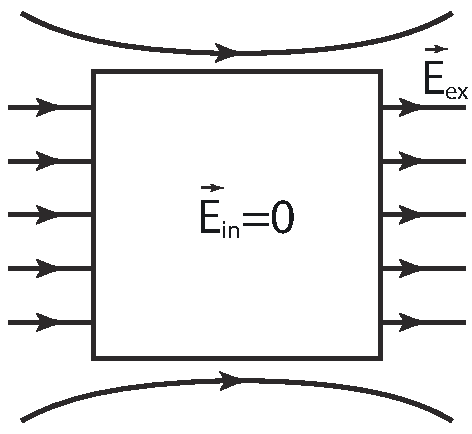
\includegraphics[width=0.47\textwidth]{lec04/solid_conductor.pdf}
        \hfill
        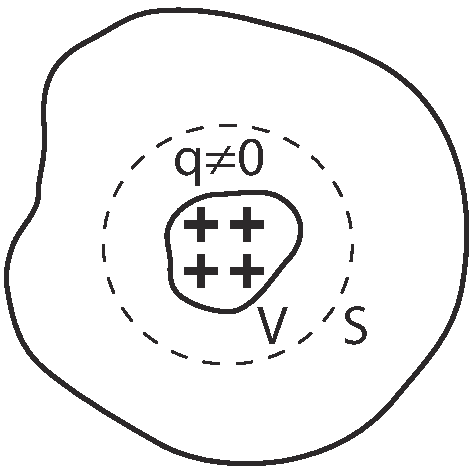
\includegraphics[width=0.47\textwidth]{lec04/solid_conductor_w-o_q.pdf}
        \parbox[t]{.47\textwidth}{
            \caption{Внутри проводника поля нет}
            \label{4:solid_conductor}
        }
        \hfill
        \parbox[t]{.47\textwidth}{
            \caption{Внутри проводника нет избыточного заряда}
            \label{4:conductor_w-o_q}
        }
    \end{figure}

    \begin{corollary}
        Вся область проводника -- эквипотенциаль.
    \end{corollary}
    \begin{proof}
         Так как \( \vec{E} = -\nabla\varphi \), то при
         \( \vec{E} \equiv 0,\ \varphi = \const \).
    \end{proof}


    \begin{corollary}
        Внутри сплошного проводника нет избыточного заряда.
    \end{corollary}
    \begin{proof}
        Допустим, что в некоторой области \( V \) внутри проводника
        \( q \ne 0 \). Эта ситуация представлена на
        рисунке~\ref{4:conductor_w-o_q}. Окружим эту область поверхностью
        \( S \). Тогда, так как \( \vec{E_{\textit{внутр}}} \equiv 0 \), то, по 
        теореме Гаусса:
        \[
            \oiint\limits_S \vec{E}\cdot\vec{dS} = \frac{q_S}{\varepsilon_0} 
            \Rightarrow q_S \equiv 0 \nonumber
        \]
    \end{proof}

\section{Поле у поверхности проводника}

    Докажем несколько утверждений:

    \begin{proposition}
        У поверхности проводника поле \( \vec{E} \) всегда перпендикулярно
        данному участку поверхности.
    \end{proposition}

    \begin{proof}
        Так как поверхность эквипотенциальна, то есть на ней
        \( \varphi = \const \), а \( \vec{E} = -\nabla\varphi \), а так как
        вектор \( \nabla\varphi \) всегда перпендикулярен поверхности уровня
        \( \varphi(x, y, z) \), то линии \( \vec{E} \) перпендикулярны
        поверхности проводника.
    \end{proof}
    \begin{comment}
        Если бы линии поля \( \vec{E} \) не были перпендикулярны поверхности 
        проводника, то \( \Delta\varphi = E\Delta l \), то есть поверхность
        была бы не эквипотенциальна, что противоречит утверждению.
    \end{comment}

    \begin{figure}[!b]
        \center
        \subfigure[Если бы поле было направлено таким образом,
                    то поверхность не была бы эквипотенциалью]{
            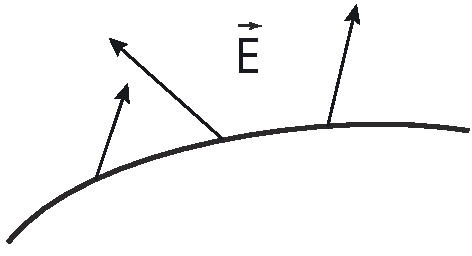
\includegraphics[width=0.3\textwidth]
                {lec04/perpendicular_field_wrong.pdf}
            \label{4:wrong}
        }
        \hfill
        \subfigure[Поле перпендикулярно поверхности проводника]{
            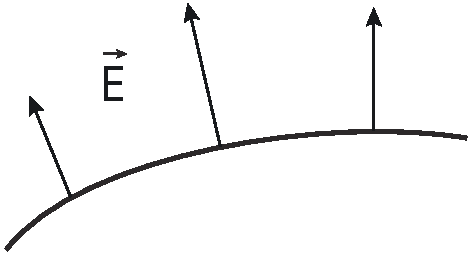
\includegraphics[width=0.3\textwidth]
                {lec04/perpendicular_field_right.pdf}
            \label{4:right}
        }
        \hfill
        \subfigure[К определению поля вблизи поверхности]{
            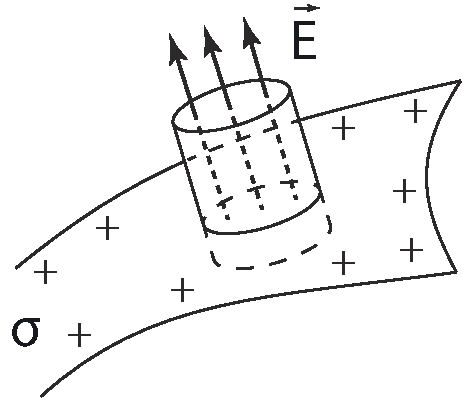
\includegraphics[width=0.3\textwidth]{lec04/conductor_surface.pdf}
            \label{4:conductor_surface}
        }
        \caption{Поле у поверхности проводника}
    \end{figure}

    \begin{proposition}
        У поверхности проводника
        \[
            \vec{E} = E_n = \frac{ \sigma }{ \varepsilon_0 },
        \]
        где \( \sigma \) -- поверхностная плотность заряда в данном месте 
        проводника.
    \end{proposition}

    \begin{proof}
        Охватим малый участок поверхности малым цилиндром. Тогда,
        по теореме Гаусса:
        \[
            \oiint\limits_S \vec{E}\cdot\vec{dS} = \frac{q_S}{\varepsilon_0} = 
            \frac{\sigma S_{\textit{тор}}}{\varepsilon_0}
        \]
        Но внутри проводника \( \vec{E} = 0 \), а вне него \( \vec{E} = E_n \), 
        следовательно
        \[
            \Phi_{S_{\textit{бок}}} = 0 \Rightarrow \oiint\limits_S \vec{E}
            \cdot \vec{dS} = ES_{\textit{тор}} \Rightarrow
            \vec{E}_{\textit{у поверхности}} = \frac{\sigma}{\varepsilon_0}.
        \]
    \end{proof}
    \begin{figure}[!b]
        \center
        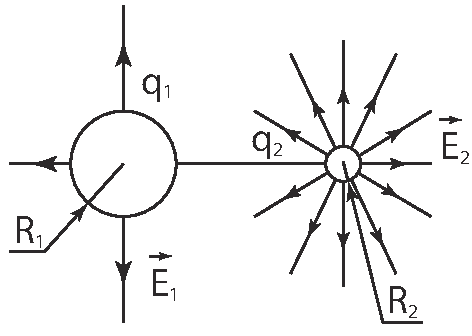
\includegraphics[width=0.47\textwidth]{lec04/E_and_R.pdf}
        \hfill
        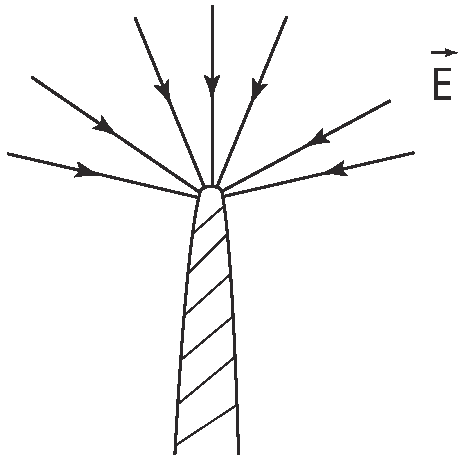
\includegraphics[width=0.47\textwidth]{lec04/needle.pdf}
        \parbox[t]{.47\textwidth}{
            \caption{Чем больше кривизна, тем сильнее поле}
            \label{4:E_and_R}
        }
        \hfill
        \parbox[t]{.47\textwidth}{
        \caption{Поле у острия иглы}
        \label{4:needle}
        }
    \end{figure}


    \begin{proposition}
        У поверхности проводника поле \( \vec{E} \) и плотность поверхностного
        заряда \( \sigma \) больше там, где больше кривизна участка поверхности
    \end{proposition}

    \begin{proof}
        Рассмотрим два металлических шара радиуса \( R_1 \) и \( R_2 \), 
        соединённых проволокой. Так как вблизи поверхности шара поле
        \[
            E = \frac{q}{4\pi\varepsilon_0 R^2},
        \]
        а потенциал металлического шара
        \[
            \varphi = \frac{q}{4\pi\varepsilon_0 R},
        \]
        то
        \[
            \varphi = ER \Rightarrow E_1 R_1 = E_2 R_2 \Rightarrow,
        \]
        и у поверхностей шаров
        \[
            \frac{E_2}{E_1} = \frac{R_1}{R_2},
        \]
        то есть
        \[
            E \sim \frac{1}{R}.
        \]
        А так как у поверхности проводника
        \[
            E = \frac{\sigma}{\varepsilon_0},
        \]
        то и
        \[
            \frac{\sigma_2}{\sigma_1} = \frac{R_1}{R_2}.
        \]
    \end{proof}

        \begin{comment}
        Пусть радиус острия иглы \( R = 10^{-6} \) м, тогда, при потенциале
        \( \varphi = 100 \) В, поле \( E \) у его поверхности
        \[
            E = \frac{\varphi}{R} = \frac{100}{10^{-6}} = 100 \cdot 10^6 =
            10^8 \frac{\text{В}}{\text{м}}.
        \]
    \end{comment}
    \begin{comment}
        При поле, большем чем \( E^{\text{возд}}_{\textit{проб}} =
        3 \cdot 10^6  (\text{В}/\text{м}) \) воздух будет пробит.
    \end{comment}

\section{Проводник с полостью в электрическом поле}
    \begin{figure}[b!]
        \center
        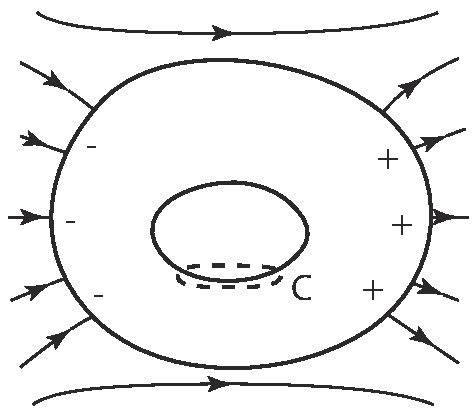
\includegraphics[width=0.47\textwidth]{lec04/holey_conductor.pdf}
        \hfill
        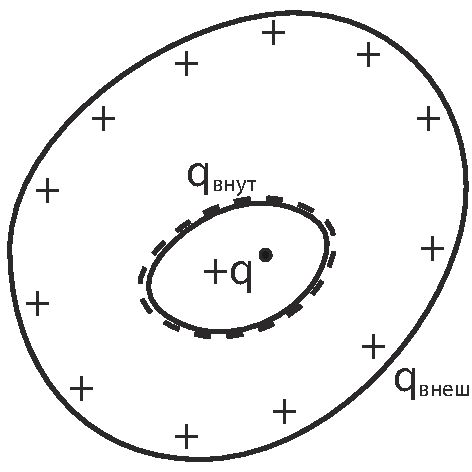
\includegraphics[width=0.47\textwidth]{lec04/q_in_ex.pdf}
        \parbox[t]{.47\textwidth}{\caption{Проводник с полостью}}
        \hfill
        \parbox[t]{.47\textwidth}{\caption{Проводник с зарядом в полости}}
    \end{figure}


    Поместим проводник с полостью во внешнее поле \( \vec{E} \). Тогда в
    полости:
    \begin{enumerate}
        \item \( \vec{E} \equiv 0 \);
        \item на внутренней поверхности полости \( \sigma \equiv 0 \).
    \end{enumerate}

    \begin{proof}
        Пусть \( \vec{E_{\textit{пол}}} \ne 0 \). А так как
        \( \vec{E_{\textit{пол}}} \) обязательно должно иметь источник, то
        \( \sigma_{\textit{пол}} \ne 0 \). % еще пикча

        Проведём контур \( C \) в полости по линии \( \vec{E} \),
        а в металле -- по любому пути. Тогда циркуляция:
        \[
            \oint\limits_C \vec{E}\cdot\vec{dl} = 
            \underbrace{\int\limits_{l_{\textit{пол}}} 
            \vec{E}_{\textit{пол}}\cdot\vec{dl}}_{\ne 0} + 
            \underbrace{\int\limits_{l_{\textit{мет}}} 
            \vec{E}_{\textit{мет}}\cdot\vec{dl}}_{= 0} \ne 0
        \]
        Но, по теореме о циркуляции поля \( \vec{E} \) следует, что
        \[
            \oint\limits_C \vec{E}\cdot\vec{dl} = 0.
        \]
        А так как \( \vec{E}_{\textit{мет}} = 0 \), то
        \( \vec{E}_{\textit{пол}} = 0 \). А так как
        \( \sigma = \varepsilon_0 E \), то и \( \sigma_{\textit{пол}} \).
    \end{proof}

 \section{Заряд в полости проводника}

    Пусть \( \vec{E}_{\textit{внеш}} = 0 \), а в полости находится заряд
    \( q \). Тогда:
    \begin{enumerate}
        \item \( q_{\textit{внутр}}^{\text{инд}} = -q \);
        \item \( q_{\textit{внеш}}^{\text{инд}} = +q \);
        \item Поле вне проводника \( \vec{E} \) создаётся только зарядом
            \( q_{\textit{внеш}}^{\text{инд}} \) на внешней поверхности и от 
            положения \( q \) в полости не зависит.
    \end{enumerate}

    \begin{proof}
    \begin{enumerate}
        \item Охватим полость замкнутой поверхностью \( S \) по металлу.
            Так как на ней \( \vec{E}_{\textit{мет}} \equiv 0 \), то:
            \[
                \oiint\limits_S \vec{E}_{\textit{мет}}\cdot\vec{dS} = 
                \frac{q_S}{\varepsilon_0} = 0 \Rightarrow q_S = q + 
                q_{\textit{внутр}}^{\text{инд}} = 0 \Rightarrow 
                q_{\textit{внутр}}^{\text{инд}} = -q
            \]
        \item Так как образец в целом нейтрален, то
            \[
                q_{\textit{внеш}}^{\text{инд}} =
                -q_{\textit{внутр}}^{\text{инд}} = +q
            \]
        \item Так как в металле \( \vec{E}_{\textit{мет}} \equiv 0 \), то  можно 
            удалить полость с зарядом \( q \) на бесконечность или залить её 
            металлом. Внешнее поле \( \vec{E} \) от этого не изменится.
    \end{enumerate}
    \end{proof}

    Таким образом, \textbf{металлическая оболочка разделяет всё пространство
    на две электронезависимых области: внутри и снаружи. Всякие изменения
    внутри не влияют на поле снаружи, и наоборот}.

    Частным вариантом оболочки является бесконечная металлическая плоскость, 
    разделяющая всё пространство на два электронезависимых полупространства.

\section{Основная задача электростатики}

    \begin{figure}[t!]
        \center
        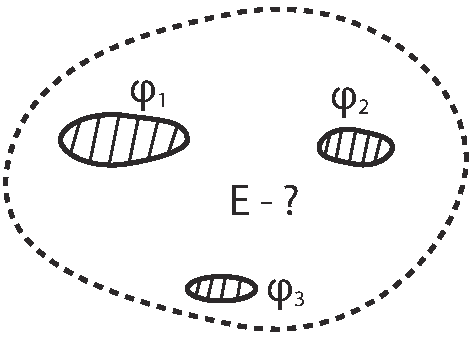
\includegraphics[width=0.5\textwidth]{lec04/E_from_phi.pdf}
        \caption{Основная задача электростатики}
    \end{figure}

    Если в пространстве известно распределение потенциала
    \( \varphi(x, y, z) \), то поле \( \vec{E} \) легко вычисляется:
    \( \vec{E} = -\nabla\varphi \).

    Основная задача электростатики формулируется так: пусть заданы геометрии
    всех проводников и диэлектриков, заданы либо заряды на них, либо их
    потенциалы. Определить поле \( \varphi(x, y, z) \) во всём пространстве.

    \begin{solution}
        Из теоремы Гаусса:
        \[
            \left\{
            \begin{array}{l}
                \div{\vec{E}} = \frac{\rho(x, y, z)}{\varepsilon_0}, \\
                \vec{E} = -\nabla\varphi.
            \end{array} \right.
        \]
        Тогда
        \[
            \div\grad\varphi = -\frac{\rho(x, y, z)}{\varepsilon_0}.
        \]

        Таким образом,
        \begin{equation}
            \label{eq4:1}
            \Delta\varphi = -\frac{\rho}{\varepsilon_0},
        \end{equation}
        Где \( \Delta \) -- оператор Лапласа.
    \end{solution}

    Уравнение (\ref{eq4:1}) называется \textit{уравнением Пуассона}. Обычно, в
    воздухе или  в вакууме, \( \rho(x, y, z) = 0 \). И тогда уравнение Пуассона
    преобразуется в уравнение Лапласа:
    \begin{equation}
        \label{eq4:2}
        \Delta\varphi = 0
    \end{equation}

    В теории дифференциальных уравнений доказывается теорема о единственности:

    \begin{theorem}
        Дифференциальное уравнение (\ref{eq4:2}) в частных производных с
        заданными граничными условиями (потенциалом или напряжённостью на
        границе области) имеет единственное решение.
    \end{theorem}

    В общем случае эта задача аналитического решения не имеет, однако, для
    некоторых симметричных зарядовых систем это решение есть. Одним из методов
    решения (\ref{eq4:2}) аналитически является \textit{метод изображений}.

\section{Метод изображений}

    \begin{figure}[t!]
        \center
        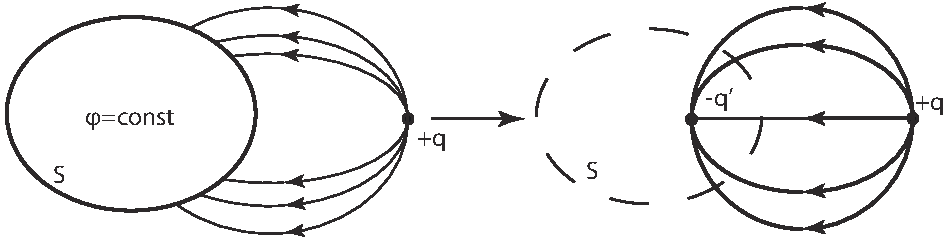
\includegraphics[width=0.7\textwidth]{lec04/images_method.pdf}
        \caption{Метод иображений}
    \end{figure}

    \begin{definition}
        \textbf{Метод изображений} -- это специальный приём расчёта
        электрического поля систем ``заряд -- металлическая поверхность''.
    \end{definition}

    Пусть задана металлическая поверхность \( S \) и заряд \( q \) вблизи неё.
    Найти либо поле \( \vec{E} \), либо потенциал \( \varphi(x, y, z) \). Тогда
    решение этой задачи методом изображений будет таково:

    Если удастся построить такую систему заряда или зарядовой конфигурации,
    которая бы вместе с исходным зарядом \( q \) создавала систему
    эквипотенциальных поверхностей, одна из которых совпадает с исходной
    поверхностью \( S \), то металлическое тело можно удалить, и при этом поле
    вне поверхности \( S \) не изменится.

    Таким образом, задача ``заряд -- металлическая поверхность'' в точности
    совпадает с задачей ``заряд -- группа зарядов''. Эта группа зарядов
    \( q_i \) называется \textit{изображением} заряда \( q \)  в поверхности
    \( S \).

    Рассмотрим работу метода изображений на примере системы ``заряд --
    металлическая плоскость'':
    \begin{figure}[b!]
        \center
        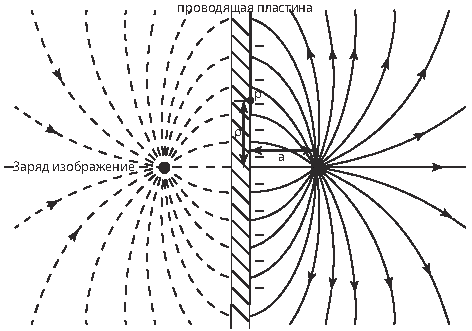
\includegraphics[width=0.7\textwidth]{lec04/flat_image.pdf}
        \caption{Применение метода изображений к системе ``заряд -- 
            металлическая плоскость''}
    \end{figure}
    \begin{example}
        На высоте \( h \) над бесконечной металлической плоскостью находится
        точечный заряд \( q \). Определить поле \( \vec{E} \) во всем верхнем
        полупространстве.
    \end{example}

    \begin{solution}
        Здесь очевидно, что эта бесконечная плоскость является эквипотенциалью 
        системы “\( +q \) -- \( -q \)”, где \( -q \) -- изображение заряда
        \( +q \) на металлическую плоскость, то есть если заменим бесконечную 
        плоскость зарядом \( -q \) на расстоянии \( h \) под плоскостью, то
        поле \( \vec{E} \) при \( z > 0 \) не изменится.

        А поле системы \( \{ q^{+}, q^{-} \} \) -- легко считается. Тогда вблизи 
        плоскости (при \( z \approx 0 \)) поле пары зарядов:
        \[
            E_{+} = \frac{q}{4\pi\varepsilon_0 {r'}^2}
        \]
        r -- расстояние от точки \( M \) до точки \( O \).Тогда результирующее
        поле:
        \[
            E_{\textit{рез}} = 2E_{+}\sin\alpha = 2E_{+}\frac{h}{r'} = 
            \frac{2qh}{4\pi\varepsilon_0(r^2 + h^2)^{\frac{3}{2}}}
        \]
        А так как \( \sigma = \varepsilon_0 E \), то распределение
        индуцированных зарядов на плоскости:
        \[
            \sigma(r) = -\frac{qh}{2\pi(r^2+h^2)^{\frac{3}{2}}}
        \]
    \end{solution}

    \begin{remark}
        Если вместо точечного заряда \( q \) над плоскостью натянут провод с 
        погонной плотностью заряда \( \gamma (\text{Кл}/\text{м})\), то
        его изображением в плоскости будет провод \( -\gamma \), а поле системы 
        ``провод -- земля'' тождественно равно полю системы ``проводник --
        проводник''.
        \[
            E_{+} = \frac{\gamma}{2\pi\varepsilon_0 r'} \nonumber
        \]
        Тогда результирующее поле:
        \[
            E = 2E_{+}\sin\alpha = 2\frac{\gamma}{2\pi\varepsilon_0 r}
            \frac{h}{r'} = \frac{\gamma h}{\pi\varepsilon_0 {r'}^2} =
            \frac{\gamma h}{\pi\varepsilon_0(r^2 + h^2)}
        \]
    \end{remark}

\section{Ёмкость уединённого проводника}

    Рассмотрим уединённый проводник. Поместим на него заряд \( q \), он 
    распределится по поверхности проводника, следовательно, появится
    электрическое поле \( \vec{E} \) и потенциал \( \varphi \) образца станет
    не равен нулю.
    \[
        \varphi = \int\limits_{\textit{поверхность}}^{\infty}
        \vec{E}\cdot\vec{dl}
    \]

    Опыт показывает, что потенциал \( \varphi \sim q \). Следовательно,
    \begin{equation}
        \label{eq4:C1}
        q = C\varphi
    \end{equation}

    \begin{definition}
        Коэффициент пропорциональности  \( C \) между зарядом проводника и его 
        потенциалом в (\ref{eq4:C1}) называется \textbf{электроёмкостью}
        проводника.
    \end{definition}

    Таким образом, по определению:
    \[
        C = \frac{q}{\varphi}
    \]

    Ёмкость измеряется в фарадах:
    \[
        C = 1\text{ Ф} = \frac{q = 1 \text{ Кл}}{\varphi = 1 \text{ В}}
    \]

    \begin{example}
        Определить радиус металлического шара с ёмкостью \( C = 1\) Ф.
    \end{example}

    \begin{solution}
        Решим эту задачу пошагово:
        \begin{enumerate}
            \item Поместим на шар заряд \( q \).
            \item Вычислим потенциал шара:
                \[
                    \varphi = \frac{q}{4\pi\varepsilon_0 R}.
                \]
            \item По определению:
                \[
                    C = \frac{q}{\varphi} = 4\pi\varepsilon_0 R.
                \]
            \item
                \[
                    R = \frac{C}{4\pi\varepsilon_0} =
                    \frac{1}{4\pi\varepsilon_0} \approx 10^10 \text{ м} =
                    10^7 \text{ км}.
                \]
        \end{enumerate}
        \end{solution}

\section{Конденсатор}
    \begin{figure}[b!]
    \center
    \subfigure[Конденсатор]{
        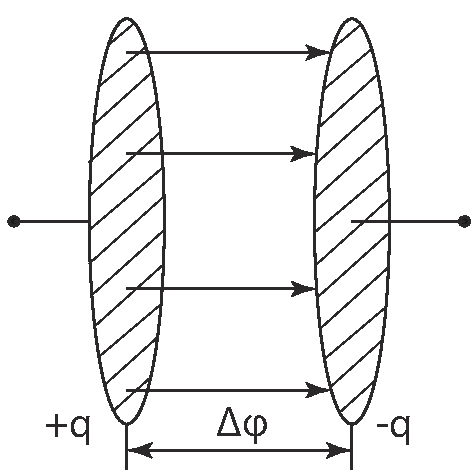
\includegraphics[width=0.3\textwidth]{lec04/capacitor.pdf}
    }
    \hfill
    \subfigure[Плоский конденсатор]{
        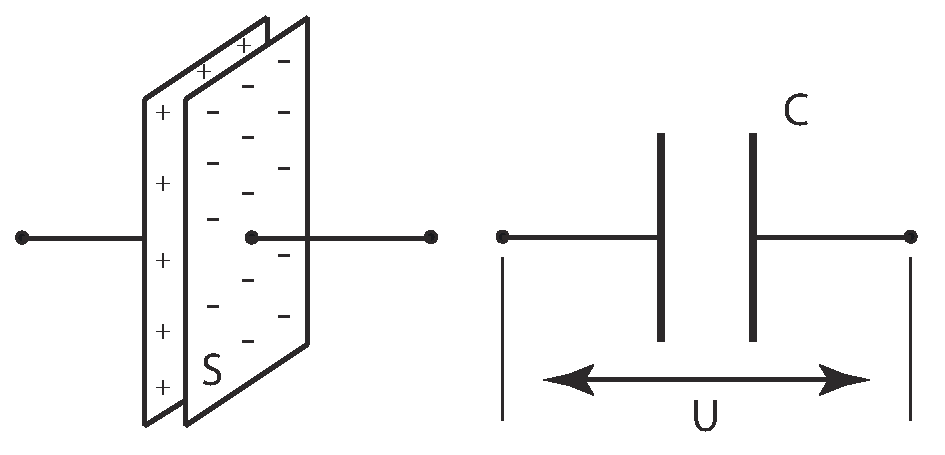
\includegraphics[width=0.6\textwidth]{lec04/flat_capacitor.pdf}
    }
    \caption{Конденсаторы}
    \end{figure}


    Если к уединённому заряженному проводнику приблизить другой, то полученная 
    система может быть использована для накопления электрического заряда.

    \begin{definition}
        Система двух близко расположенных проводников называется
        \textbf{конденсатором}.
    \end{definition}

    Выражение ``зарядить конденсатор'' означает внесение на его обкладки равные
    заряды \( +q \) и \( -q \), где \( q = +q = |-q| \) -- называется зарядом
    конденсатора. Опыт показывает, что \( \Delta\varphi \sim q \), или:
    \begin{equation}
        \label{eq4:C2}
        q = C \Delta\varphi
    \end{equation}

    \begin{definition}
        Коэффициент пропорциональности \( C \) между зарядом конденсатора и его
        разностью потенциалов на его обкладках в (\ref{eq4:C2}) называется
        \textbf{ёмкостью} конденсатора. Таким образом, по определению,
        \[
            C \equiv \frac{q}{\Delta\varphi}.
        \]
    \end{definition}

    \begin{remark}
        Разность потенциалов \( \Delta\varphi \) называется \textbf{напряжением}
        на конденсаторе \( U = \Delta\varphi \). Таким образом,
        \[
            C = \frac{q}{U}.
        \]
    \end{remark}

    Так как фарад величина очень большая (\textit{ёмкостью 1 Ф обладал бы 
    уединённый шар, радиус которого больше, чем 10 радиусов Солнца}), то на 
    практике используют производные величины от фарада: \( 1\text{ мкФ} =
    1 \cdot 10^{-6}\text{ Ф} \), \( 1\text{ нФ} = 1 \cdot 10^{-9}\text{ Ф} \),
    \( 1\text{ пФ} = 1 \cdot 10^{-12}\text{ Ф} \).

        \begin{definition}
        Конденсатор называется \textbf{плоским}, если его обкладками являются
        пара близких параллельных плоскостей. % пикча
    \end{definition}

    Вычислим ёмкость плоского конденсатора (\( S, d \)). % пикча 1 & 2
    \begin{enumerate}
        \item Зарядим конденсатор.
        \item Вычислим поле \( \vec{E} \) между обкладками.
        Так как каждая заряженная плоскость создаёт вокруг себя поле
        \[
            E = \frac{\sigma}{2\varepsilon_0},
        \]
        то их суммарное поле равно
        \[
            E = \frac{\sigma}{\varepsilon_0}.
        \]
         Это и есть поле в конденсаторе:
         \[
             E = \frac{\sigma}{\varepsilon_0} = \frac{q}{\varepsilon_0 S}.
         \]
        \item Вычислим напряжение:
            \[
                U = \Delta\varphi = Ed = \frac{qd}{\varepsilon_0 S}.
            \]
        \item По определению:
        \[
            C = \frac{q}{U} = \frac{q\varepsilon_0 S}{qd} =
            \frac{\varepsilon_0 S}{d}.
        \]
    \end{enumerate}

    \begin{example}
        Вычислить ёмкость плоского конденсатора, площадь обкладок которого
        \( S = 1 \text{м}^2\) и расстояние между ними \( d = 10^{-6} \) м.
    \end{example}

    \begin{solution}
        \[
            C = \frac{\varepsilon_0 S}{d} = \frac{10^{-11} \cdot 1}{10^{-6}} =
            10^{-5} \text{ Ф} = 10 \text{ мкФ}
        \]
    \end{solution}

    \begin{example}
        Вычислить погонную ёмкость цилиндрического конденсатора (коаксиальной
        линии), если радиусы цилиндров \( R_2 \) и \( R_1 \) такие, что 
        \( R_2 > R_1 \), а длина цилиндров \( l \gg R_2 \).
    \end{example}

    \begin{figure}[t!]
        \center
        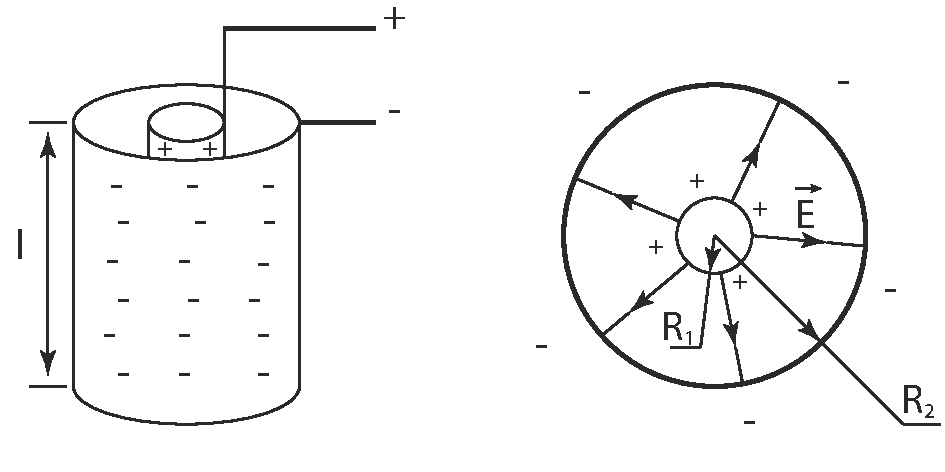
\includegraphics[width=0.6\textwidth]{lec04/cylinder_capacitor.pdf}
        \caption{Цилиндрический конденсатор}
    \end{figure}

    \begin{solution}
        \begin{enumerate}
            \item Заряжаем конденсатор до заряда \( q = \gamma l \).
            \item Поле между цилиндрами, то есть \( R_1 < r < R_2 \):
            \[
                 E = \frac{\gamma}{2\pi\varepsilon_0 r}.
            \]
            \item Напряжение:
            \[
                U = \Delta\varphi = \int\limits_{R_1}^{R_2} Edr = 
                \int\limits_{R_1}^{R_2} \frac{\gamma}{2\pi\varepsilon_0 r}dr = 
                \frac{\gamma}{2\pi\varepsilon_0}\ln\frac{R_2}{R_1} = 
                \frac{q}{2l\pi\varepsilon_0}\ln\frac{R_2}{R_1}.
            \]
            \item Ёмкость:
            \[
                C = \frac{q}{U} =
                \frac{q \cdot 2l\pi\varepsilon_0 } {q\ln\frac{R_2}{R_1}} = 
                \frac{2\pi\varepsilon_0 l}{\ln\frac{R_2}{R_1}}.
            \]
            \item Погонная ёмкость коаксиальной линии:
            \[
                C_0 = \frac{C}{l} = \frac{2\pi\varepsilon_0}{\ln\frac{R_2}{R_1}} 
                \left(\frac{\text{Ф}}{\text{м}}\right).
            \]
        \end{enumerate}
    \end{solution}

\section{Соединение конденсаторов}

    \begin{figure}[b!]
        \center
        \subfigure[Параллельно]{
            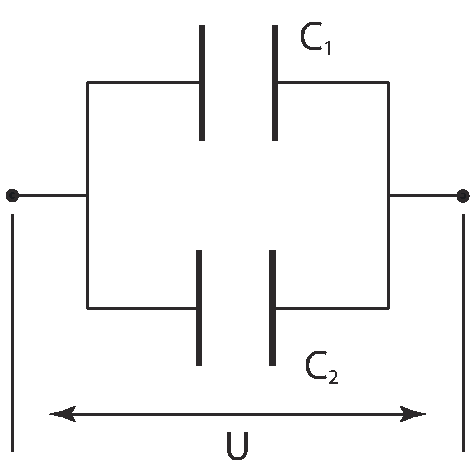
\includegraphics[width=0.47\textwidth]{lec04/C_parallel.pdf}
        }
        \hfill
        \subfigure[Последовательно]{
            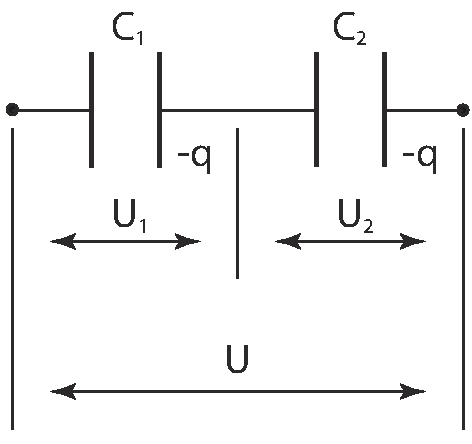
\includegraphics[width=0.47\textwidth]{lec04/C_serial.pdf}
        }
        \caption{Соединения конденсаторов}
    \end{figure}
    \begin{enumerate}
        \item Параллельное:
        \begin{align}
        \left\{
        \begin{array}{rl}
            q_{ab} = & q_1 + q_2 \\
            U_{ab} = & U_1 = U_2
        \end{array} \right. \nonumber \\
        C_{ab} = C_1 + C_2 \nonumber
        \end{align}
        \item Последовательное: % пикча
        \begin{align}
        \left\{
        \begin{array}{rl}
            U_{ab} = & U_1 + U_2 \\
            q_{ab} = & q_1 = q_2
        \end{array} \right. \nonumber \\
        \frac{1}{C_{ab}} = \frac{1}{C_1} + \frac{1}{C_2} \nonumber
        \end{align}
    \end{enumerate}

\section{Энергия заряженного конденсатора}

    %пикча
    Pарядка конденсатора -- это процесс разделение зарядов, для проведения
    которого необходимо совершать работу против поля \( \vec{E} \).

    Пусть \( q' \) -- текущий заряд на обкладках, \( \vec{E}' \) -- текущее
    поле в процессе зарядки, \( U' \) -- текущее напряжение, \( dq' \) --
    очередная порция переносимого заряда каким-либо внешним устройством 
    (генератором).

    Тогда элементарная работа внешних сил по переносу очередной порции заряда
    \( dq' \) с левой обкладки на правую, с более высоким потенциалом, по 
    определению может быть вычислена как \( dA = U' dq' \), а поскольку
    \( U' = \frac{q'}{C} \), то энергия заряженного конденсатора до его полной 
    зарядки, то есть до скопления зарядов \( q \) и \(-q \) на обкладках:
    \[
        W = A = \int\limits_0^q \frac{q' dq'}{C} = \frac{q^2}{2C}
    \]
    А так как \( q = CU \), то:
    \begin{equation}
        \label{eq4:C3}
        W = \frac{CU^2}{2}
    \end{equation}

    \begin{figure}[b!]
        \center
        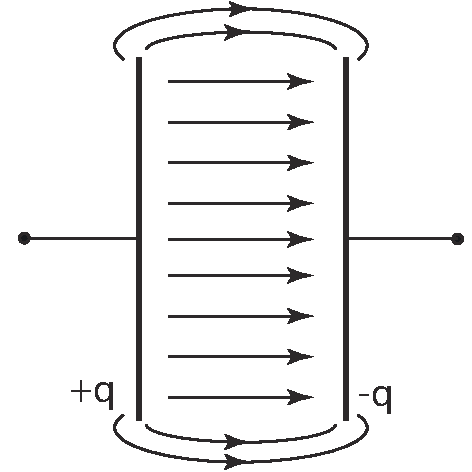
\includegraphics[width=0.47\textwidth]{lec04/flat_capacitor_field.pdf}
        \caption{Поле плоского конденсатора}
    \end{figure}

\section{Локализация энергии в электростатическом поле}

    % пикча
    Рассмотрим плоский конденсатор \( C \):
    \[
        C = \frac{\varepsilon_0 S}{d}.
    \]
    Энергия \( W \), накопленная в нем:
    \[
        W = \frac{CU^2}{2}.
    \]
    Эта энергия локализована в электрическом поле между обкладками конденсатора.
    Вычислим её плотность
    \[
        w = \frac{W}{V} \, \left(\frac{\text{Дж}}{\text{м}^3}\right).
    \]

    Так как \( U = Ed\) и \( C = \frac{\varepsilon_0 S}{d} \), то:
    \[
        W = \frac{\varepsilon_0 S}{2d} \cdot E^2 d^2 =
        \frac{\varepsilon_0 S E^2 d}{2} = [ S \cdot d = V_E ] =
        \frac{\varepsilon_0 E^2}{2} V_E,
    \]
    где \( V_E \) -- объем, занимаемый электрическим полем. В случае плоского 
    конденсатора \( V_E = V \).

    Тогда,
    \[
        w = \frac{\varepsilon_0 E^2}{2}.
    \]
